\section[Flux du champ électrostatique]{Flux du champ électrostatique.\\Théorème de Gauss}

    \subsection{Charge ponctuelle : flux à travers une sphère}

        On considère une charge ponctuelle $Q$ en un point $O$ et une sphère $S$ de rayon $r$ de centre $O$. On note
        \begin{equation}
            \vec{E}=\frac{Q}{4\pi\varepsilon_{0}r^{2}}\vec{u_r}.
        \end{equation}
        Alors en notant $\vec{n}^{\text{ext}}$ le vecteur normal à la surface $S$,
        \begin{equation}
            \boxed{
                \oiint_{S}\vec{E}\cdot\vec{n}^{\text{ext}}\rmd S=\frac{Q}{4\pi\varepsilon_{0}r^{2}}\oiint\rmd S=\frac{Q}{\varepsilon_{0}}.
            }
        \end{equation}

    \subsection{Théorème de Gauss}
        \subsubsection{Une charge ponctuelle à l'intérieur d'une surface fermée}

            Soit $V$ un volume quelconque de l'espace contenant une charge $Q$. On note $S$ une sphère centrée en $Q$ contenue dans $V$, et $S'$ le reste de la surface correspondant à $V$.En un point $M$ quelconque du volume, on a
            \begin{equation}
                \vec{E}(M)=\frac{Q}{4\pi\varepsilon_{0}r^{2}}\vec{u_r}.
            \end{equation}

            On a 
            \begin{equation}
                \oiint_{S\cup S'}\vec{E}\cdot\vec{n}^{\text{ext}}\rmd S=\iiint_{V}\div\vec{E}\rmd V,
            \end{equation}
            et pour un problème à symétrie sphérique, on a pour tout $r\neq0$,
            \begin{equation}
                \div\vec{E}=\frac{1}{r^{2}}\frac{\partial}{\partial r}\left(r^{2}E_r\right).
            \end{equation}
            Ainsi, $\div\vec{E}=0$ pour tout $r\neq 0$, d'où 
            \begin{align}
                \iiint_{V}\div\vec{E}\rmd V=0=\oiint_{S}\vec{E}\cdot\vec{n}^{\text{ext}}\rmd S+\oiint_{S'}\vec{E}\cdot\vec{n}^{\text{ext}}\rmd S',
            \end{align}
            et les deux normales extérieures sont opposées l'une de l'autre. Finalement,
            \begin{equation}
                \oiint_{S}\vec{E}\cdot\vec{n}^{\text{ext}}\rmd S=\oiint_{S}\vec{E}\cdot\vec{u_r}\rmd S'=\frac{Q}{\varepsilon_{0}}.
            \end{equation}

            Ainsi, si une surface $S$ contient une charge $Q$, on a toujours
            \begin{equation}
                \boxed{
                    \oiint_{S}\vec{E}\cdot\vec{n}^{\text{ext}}\rmd S=\frac{Q}{\varepsilon_{0}}.
                }
            \end{equation}

        \subsubsection{Charge ponctuelle à l'extérieur d'une surface fermée}

            Dans ce cas, on a directement
            \begin{equation}
                \boxed{
                    \oiint_{S}\vec{E}\cdot\vec{n}^{\text{ext}}\rmd S=\iiint_{V}\div\vec{E}\rmd V=0.
                }
            \end{equation}

        \subsubsection{Bilan}

            Si $\vec{E}$ est le champ total créé par $N$ charges $Q_i$, alors
            \begin{equation}
                \boxed{
                    \oiint_{S}\vec{E}\cdot\vec{n}^{\text{ext}}\rmd S=\frac{Q^{\text{int}}}{\varepsilon_{0}}.
                }
            \end{equation}

            Ici, $Q^{\text{int}}$ est la somme de toutes les charges qui sont à l'intérieur de la surface $S$.

    \subsection{Comment appliquer le théorème de Gauss}

        Le but est de calculer des champs électrostatiques $\vec{E}$ dans des cas de hautes symétries. La méthode est la suivante:
        \begin{itemize}
            \item [($\alpha$)] Invariance et symétries : donne la géométrie de $\vec{E}$;
            \item [($\beta$)] Choisir une surface de Gauss adaptée (ou bien $\vec{E}\parallel\vec{n}^{\text{ext}}$ avec $E$ qui est constant sur la surface ou bien $\vec{E}\perp\vec{n}^{\text{ext}}$) avec un dessin;
            \item [($\gamma$)] Conclure.
        \end{itemize}

    \subsection{Exemples fondamentaux}
        \subsubsection{Sphère uniformément chargée en volume ou en surface}

            On considère le système donnée à la Figure~\ref{fig:sphere_uniformement_chargee_volume_surface}.
            \begin{figure}
                \centering
                \tikzsetnextfilename{sphere_uniformement_chargee_volume_surface}
                \begin{tikzpicture}[scale=1]  
                    % \helpgrid{3}{3}
                    \coordinate (O) at (0,0);
                    \node at (O) {$\bullet$};
                    \node at (O) [left] {O};
                    \coordinate (A) at (2,2);
                    \draw [->, -stealth] (O)--(0,2.5) node [above] {z};
                    \draw[dashed] (O)--(A) node [below, midway, shift={(0.2,-0.1)}] {$r$};
                    \node at (A) {$\bullet$};
                    \node at (A) [above] {M};
                    \draw [->] (0,0.75) to [bend left=45] (0.5,0.5) node [above] {$\theta$};
                    \draw [->] (-0.25,2.3) to [bend right=90] (0.25,2.3) node [right] {$\varphi$};
                    \draw [pattern=north east lines, opacity=0.25] (O) circle (1.5);
                    \draw[<->] (O)--(-45:1.5) node [below, midway] {$R$};
                \end{tikzpicture}
                \caption{Sphère uniformément chargée en volume ou en surface.}    
                \label{fig:sphere_uniformement_chargee_volume_surface}
            \end{figure}

            \begin{itemize}
                \item [($\alpha$)] Toute rotation d'axe passant par O laisse la distribution invariant, donc 
                \begin{equation}
                    \vec{E}(r,\theta,\varphi)=\vec{E}(r)=\begin{pmatrix}
                        E_r(r)\\ E_{\theta}(r)\\E_{\varphi}(r)
                    \end{pmatrix}.
                \end{equation}
                Les plans $(M,\vec{u_r},\vec{u_{\varphi}})$ et $(M,\vec{u_r},\vec{u_{\theta}})$ sont des PS valable pour tout point $M$. Ainsi, $\vec{E}$ est radial et $\vec{E}(M)=E(r)\vec{u_r}$.
                \item [($\beta$)] La bonne surface de Gauss est une sphère de centre $O$ et de rayon $r$ variable.
                \item [($\gamma$)] On a 
                \begin{equation}
                    \oiint_{S}\vec{E}\cdot\vec{n}^{\text{ext}}\rmd R=\oiint_{S}E(r)\rmd S=E(r)4\pi r^{2}=\frac{Q_{\text{int}}(r)}{\varepsilon_{0}}.
                \end{equation}
                Ainsi,
                \begin{equation}
                    \boxed{
                        \vec{E}(r)=\frac{Q_{\text{int}}(r)}{4\pi\varepsilon_{0}r^{2}}\vec{u_r}.
                    }
                \end{equation}
            \end{itemize}

            \paragraph{Boule uniformément chargée en volume.}

                La densité $\rho$ est constante et vaut $\frac{Q}{\frac{4}{3}\pi R^{3}}$ où $Q$ est la charge présente dans l'entièreté de la boule. Ainsi, pour $r\geqslant R$, on a 
                \begin{equation}
                    Q_{\text{int}}(r\geqslant R)=Q,
                \end{equation}
                d'où
                \begin{equation}
                    \boxed{
                        \vec{E}(r\geqslant R)=\frac{Q}{4\pi\varepsilon_0 r^{2}}\vec{u_r}.
                    }
                \end{equation}

                Si $r\leqslant R$, alors on a 
                \begin{equation}
                    Q_{\text{int}}(r\leqslant R)=\iiint \rho\rmd V=\rho\frac{4}{3}\pi r^{3}=Q\left(\frac{r}{R}\right)^{3}.
                \end{equation}
                Ainsi, on a 
                \begin{equation}
                    \boxed{
                        \vec{E}(r\leqslant R)=\frac{Qr}{4\pi\varepsilon_0 R^{3}}\vec{u_r}=\frac{Q}{4\pi\varepsilon_0 R^{2}}\left(\frac{r}{R}\right)\vec{u_r}.
                    }
                \end{equation}

            \paragraph{Sphère uniformément chargée en surface.}

                Pour $r>R$, on a le même résultat que précédemment. Pour $r<R$, on a $Q_{\text{int}}(r<R)=0$, donc $\vec{E}(r<R)=\vec{0}$. $\vec{E}$ est donc discontinu à la surface de la sphère (variation d'amplitude égal à $\sigma/\varepsilon_{0}$). C'est un modèle non physique.                

        \subsubsection{Cylindre infini uniformément chargé en volume ou en surface}

            On considère un cylindre de rayon $R$ d'axe $(Oz)$.
            La distribution de charge est à symétrie cylindrique \og infinie\fg. 

            \begin{itemize}
                \item [($\alpha$)] Il y a une symétrie de révolution par rapport à l'axe $(Oz)$ et une invariance par translation parallèlement à l'axe $(Oz)$. De plus, tout plan perpendiculaire à $(Oz)$ est un plan de symétrie. Enfin, tout plan contenant $(Oz)$ est un plan de symétrie. Finalement, on a 
                \begin{equation}
                    \boxed{
                    \vec{E}(M)=E(r)\vec{u_r}.
                    }
                \end{equation}
                \begin{remark}
                    Si la distribution est non infinie, a priori on a 
                    \begin{equation}
                        \vec{E}(M)=\begin{pmatrix}
                            E_r(r,z)\\0\\e_z(r,z)
                        \end{pmatrix}.
                    \end{equation}
                \end{remark}

                \item [$(\beta$)] La surface de Gauss que l'on prend est un cylindre d'axe $(Oz)$ de rayon $r$, de hauteur de $h$, formé par deux disques perpendiculaires à l'axe $(Oz)$.
                
                \item [$(\gamma)$] Le théorème de Gauss donne
                \begin{equation}
                    \oiint_{S}\vec{E}\cdot\vec{n}^{\text{ext}}\rmd S=\frac{Q_{\text{int}}(r)}{\varepsilon_{0}},
                \end{equation}
                où $S=\Sigma\cup S_1\cup S_2$ où $S_1$ et $S_2$ correspondent aux disques. Ainsi, 
                \begin{equation}
                    \oiint_{S}\vec{E}\cdot\vec{n}^{\text{ext}}\rmd S=0+0+\iint_{\Sigma}E(r)\vec{u_r}\cdot\vec{n}^{\text{ext}}\rmd \Sigma=E(r)\times 2\pi r h.
                \end{equation}
                Ainsi,
                \begin{equation}
                    \boxed{
                        E(r)=\frac{Q_{\text{int}}(r)}{2\pi\varepsilon_{0}hr}.
                    }
                \end{equation}

            \end{itemize}

            \paragraph{Cylindre uniformément charge en volume.} 
            
                On considère une tranche d'hauteur $h$, on a $Q=\rho h\pi R^{2}$. On introduit donc 
                \begin{equation}
                    \boxed{
                        \lambda=\frac{Q}{h}=\rho\pi R^{2}.
                    }
                \end{equation}
                C'est la charge linéique en \si{\coulomb\per\metre}. Pour $r\geqslant R$, on a $Q_{\text{int}}(r\geqslant R)=\lambda h$, d'où 
                \begin{equation}
                    \boxed{
                        \vec{E}(r\geqslant R)=\frac{\lambda}{2\pi\varepsilon_{0}r}\vec{u_r}.
                    }
                \end{equation}

                Si $r\leqslant R$, on a $Q_{\text{int}}(r\leqslant R)=\rho \pi r^{2}h=\lambda h\left(\frac{r}{R}\right)^{2}$. Ainsi,
                \begin{equation}
                    \boxed{
                        \vec{E}(r\leqslant R)=\frac{\lambda r}{2\pi\varepsilon_{0}R^{2}}\vec{u_r}.
                    }
                \end{equation}

            \paragraph{Cylindre uniformément chargé en surface.} 

                Si $r<R$, on a $\vec{E}(r<R)=\vec{0}$. Si $r>R$, on a $Q_{\text{int}}(r>R)=Q=\lambda h$, donc $\vec{E}(r>R)=\frac{\lambda}{2\pi\varepsilon_{0}r}\vec{u_r}$. À nouveau, il y a une discontinuité égale à $\sigma/@\varepsilon_{0}$ avec $\sigma=\frac{\lambda}{2\pi R}$. Elle est due au modèle surfacique.

            
        \subsubsection{Plan infini uniformément chargé en surface}

            On considère le système décrit à la Figure~\ref{fig:plan_uniformement_charge_surface}.
            \begin{figure}
                \centering
                \tikzsetnextfilename{plan_uniformement_charge_surface}
                \begin{tikzpicture}[scale=1]  
                    % \helpgrid{3}{3}
                    \coordinate (A) at (-2,-0.5);
                    \coordinate (B) at (-1.5,0);
                    \node at (0,0) [below right]{O};
                    \draw [->,-latex] (0,0) --++ (-0.5,-1) node [below] {x};
                    \draw [->,-latex] (0,0) --++ (1.5,0) node [right]{y};
                    \draw [->,-latex] (0,0) --++ (0,1.5) node [above]{z};

                    \draw (-4,-1) -- (-3,1) -- (5,1) -- (4,-1) -- cycle;

                    \node at (3,-0.5) {$\sigma$};
                  
                    \filldraw [fill=gray!20, opacity=0.4] (A) --++ (1,0) --++ (0,2) --++ (-1,0) -- cycle;
                    \filldraw [fill=gray!30, opacity=0.4] (B) --++ (1,0) --++ (0,2) --++ (-1,0) -- cycle;
                    \draw[opacity=0.4] (A) -- (B);
                    \draw[opacity=0.4] ($(A)+(1,0)$) -- ($(B)+(1,0)$);
                    \draw[opacity=0.4] ($(A)+(1,2)$) -- ($(B)+(1,2)$);
                    \draw[opacity=0.4] ($(A)+(0,2)$) -- ($(B)+(0,2)$);

                    \filldraw [fill=gray!20, opacity=0.4,dashed] (A) --++ (1,0) --++ (0,-2) --++ (-1,0) -- cycle;
                    \filldraw [fill=gray!30, opacity=0.4, dashed] (B) --++ (1,0) --++ (0,-2) --++ (-1,0) -- cycle;
                    \draw[opacity=0.4, dashed] ($(A)+(1,-2)$) -- ($(B)+(1,-2)$);
                    \draw[opacity=0.4, dashed] ($(A)+(0,-2)$) -- ($(B)+(0,-2)$);

                    \fill[pattern=north east lines, pattern color=blue] (A)--++(1,0)--($(B)+(1,0)$)--(B)--cycle;
                    \node[text=blue] at ($(A)+(-0.5,0)$) {$\sigma_S$};
                \end{tikzpicture}
                \caption{Plan uniformément chargé en surface.}    
                \label{fig:plan_uniformement_charge_surface}
            \end{figure}

            Par plan infini, on entend que les longueurs caractéristiques du plan selon les axes $x$ et $y$ sont très grandes devant l'épaisseur du plan : $L_x,L_y\gg e$.

            \begin{itemize}
                \item [($\alpha$)] Il y a invariance par translation par rapport aux axes $(Ox)$ et $(Py)$. Ainsi, le champ ne dépend pas de $x$ ni de $y$. Pour les symétries, tout plan parallèle à $(xOy)$ est un PS, donc $E_y=0$. Tout plan parallèle à $(yOz)$ est un PS, donc $E_x=0$. Ainsi, on a $\vec{E}(M)=E(z)\vec{u}_z$.
                Enfin, le fait que la plan $(xOy)$ est un PS implique $E(-z)=-E(z)$.

                \item [($\beta$)] La surface de Gauss est un cylindre de générateur parallèle à $(Oz)$, de hauteur 2z centré sur le plan $z=0$.
                
                \item [($\gamma$)] On a 
                \begin{align}
                    \oiint_{S=S_1\cup S_2\cup \Sigma}\vec{E}\cdot\vec{n}^{\text{ext}}\rmd S
                    &=\frac{Q_{\text{int}}}{\varepsilon_0},\\
                    &=\frac{\sigma S}{\varepsilon_0},\\
                    &=0+\iint_{S_1}E(z)\vec{u}_z\cdot\vec{u}_z\rmd S\\
                    &\quad+\iint_{S_2}E(-z)\vec{u}_z\cdot\left(-\vec{u}_z\right)\rmd S,\\
                    &=
                    E(z)S+E(z)S.
                \end{align}
                Ainsi, 
                \begin{equation}
                    \boxed{\vec{E}(z>0)=\frac{\sigma}{2\varepsilon_0}\vec{u}_z,}
                \end{equation}
                et 
                \begin{equation}
                    \boxed{\vec{E}(z<0)=-\frac{\sigma}{2\varepsilon_0}\vec{u}_z.}
                \end{equation}
                
                La différence en $z=0$ vaut $\frac{\sigma}{\varepsilon_0}$.
            \end{itemize}

            \paragraph{Couche de charges infinie uniformément chargée en volume.}

                On se réfère à la Figure~\ref{fig:couche_charge_uniformement_chargee_volume}.

                \begin{figure}
                    \centering
                    \tikzsetnextfilename{couche_charge_uniformement_chargee_volume}
                    \begin{tikzpicture}[scale=1]  
                        % \helpgrid{3}{3}
                    \node at (0,0) [below left]{O};
                    \draw (0,0) circle (0.1) node [below right] {x} node {$\cdot$};
                    \draw [->,-latex] (0,0) --++ (1.5,0) node [right]{y};
                    \draw [->,-latex] (0,0) --++ (0,1.5) node [above]{z};

                    \draw (-3,-1)--++(6,0);
                    \draw (-3,1)--++(6,0);
                    \draw[latex-latex] (-3.1,-1)--++(0,2) node [midway, left] {$e$};
                    \node at (4,0) {$\rho$ = constante};
                    \draw[dashed, draw=blue] (-2.5,0) rectangle++(1,3);
                    \draw[latex-latex] (-2.5,3.2)--++(1,0) node [midway, above] {$S$};
                    \end{tikzpicture}
                    \caption{Couche de charges infinie uniformément chargée en volume.}    
                    \label{fig:couche_charge_uniformement_chargee_volume}
                \end{figure}

                \begin{enumerate}
                    \item [($\alpha$)] Il y a invariance par translation selon $(Ox)$ et $(Oy)$, donc $\vec{E}$ ne dépend ni de $x$, ni de $y$. Les symétries sont les mêmes que précédemment, on a donc $\vec{E}(M)=E(z)\vec{u}_z$ et $E(-z)=-E(z)$.
                    \item [($\beta$)] La surface de Gauss est la même que précédemment, mais avec la base dans le plan $z=0$.
                    \item [($\gamma$)] On a donc 
                    \begin{equation}
                        \oiint_{S}\vec{E}\cdot\vec{n}^{\text{ext}}\rmd S=0+0+E(z)\times S=\frac{Q_{\text{int}}(z)}{\varepsilon_0}.
                    \end{equation}

                    Si $z\geqslant e/2$, on a $Q_{\text{int}}(z\geqslant e/2)=\rho\times S\times e/2$, donc 
                    \begin{equation}
                        \boxed{
                        E(z\geqslant e/2)=\frac{\rho e}{2\varepsilon_0},\qquad E(z\leqslant -e/2)=-\frac{\rho e}{2\varepsilon_0}.}
                    \end{equation}
                    Si $0\leqslant z\leqslant e/2$, on a $Q_{\text{int}}(z)=\rho\times S\times z$, donc 
                    \begin{equation}
                        \boxed{
                        E(0\leqslant z\leqslant e/2)=\frac{\rho z}{\varepsilon_0},\qquad E(-e/2\leqslant z\leqslant 0)=-\frac{\rho z}{\varepsilon_0}.}
                    \end{equation}
                    Ainsi, $E$ est continu. Dans le limite $e\to0$, on retrouve le modèle de la nappe de charges avec $\rho e=\sigma$ fini.
                \end{enumerate}

    \subsection{Condensateur plan sans effet de bord. Capacité}
        \subsubsection{Condensateur plan sans effet de bord}

            Le condensateur plan est constitué de deux armatures métalliques se faisant face, séparées par un isolant ou un diélectrique. On se réfère à la Figure~\ref{fig:condensateur_plan_sans_effet_de_bord}.
            \begin{figure}
                \centering
                \tikzsetnextfilename{condensateur_plan_sans_effet_de_bord}
                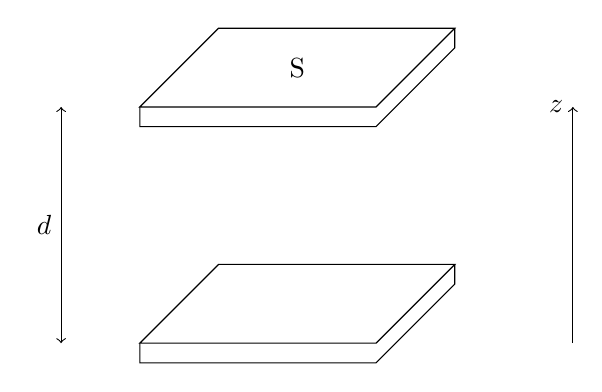
\begin{tikzpicture}[scale=1]  
                    \draw (0,0) --++ (1,1) --++ (3,0) --++ (-1,-1) -- cycle;
                    \draw (0,0) --++ (0,-0.25) --++ (3,0) --++ (1,1) --++ (0,0.25);
                    \draw (0,3) --++ (1,1) --++ (3,0) --++ (-1,-1) -- cycle;
                    \draw (0,3) --++ (0,-0.25) --++ (3,0) --++ (1,1) --++ (0,0.25);                    
                    \draw[<->](-1,0)--++(0,3) node [left, midway] {$d$};
                    \draw[->] (5.5,0)--++(0,3) node [left] {$z$};
                    \node at (2, 3.5) {S};
                \end{tikzpicture}
                \caption{Condensateur plan sans effet de bord.}    
                \label{fig:condensateur_plan_sans_effet_de_bord}
            \end{figure} 

            On fait l'hypothèse que $d\ll\sqrt[]{S}$, ce qui correspond au fait que les armatures sont \og infinies\fg : il n'y a pas d'effet de bords. Chaque armature est donc un plan infini sans épaisseur.

            Les deux plans sont soumis à une tension $U$ : il y a une accumulation de charges opposées sur les deux plans en regard.

        \subsubsection{Champ électrique}

            \begin{enumerate}
                \item [($\alpha$)] Il y a invariance par translation sur $(Ox)$ et $(Oy)$, donc $\vec{E}(M)=\vec{E}(z)$. Tout plan parallèle à $(xOz)$ et $(yoZ)$ est un PS, donc $E_x=E_y=0$. Finalement,
                \begin{equation}
                    \vec{E}(M)=E(z)\vec{u}_z.
                \end{equation}
                Ainsi, $\vec{E}$ est perpendiculaire aux armatures. Si $\vec{\rmd l}$ est un déplacement infinitésimal sur l'armature, on a 
                \begin{equation}
                    \vec{E}\cdot\vec{\rmd l}=0=-\rmd V=-\left[
                        \frac{\partial V}{\partial x}\rmd x+\frac{\partial V}{\partial y}\rmd y+0
                    \right].
                \end{equation}
                Donc $\frac{\partial V}{\partial x}=\frac{\partial V}{\partial x}=0$ sur une armature, donc $V$ est constant sur une armature. On note $V_1$ le potentiel de l'armature située en $z=d/2$ et $V_2$ celle en $z=-d/2$. On a $U=V_1-V_2$. Or $V$ est défini ) une constante près. On choisit donc $V_1=U/2$ et $V_2=-U/2$. Cela entraîne donc que le plan $z=0$ est un PAS. Donc les charges (surfaciques) valent $+\sigma$ sur l'armature haute, et $-\sigma$ sur l'armature basse. On applique le théorème de superposition comme selon la Figure~\ref{fig:theoreme_superposition_armature_condensateur_plan}.
                \begin{figure}
                    \centering
                    \tikzsetnextfilename{theoreme_superposition_armature_condensateur_plan}
                    \begin{tikzpicture}[scale=0.9]  
                        \draw (0,0) --++ (1,1) --++ (3,0) --++ (-1,-1) -- cycle;
                        \draw (0,3) --++ (1,1) --++ (3,0) --++ (-1,-1) -- cycle;
                        \node[text=red] at (2, -0.5) {$\vec{0}$};
                        \node[text=red] at (2, 4.5) {$\vec{0}$};
                        \node[text=red] at (2, 2) {$-\dfrac{\sigma}{\varepsilon_0}\vec{u_z}$};
                        \node at (0,3) [left] {$+\sigma$};
                        \node at (0,0) [left] {$-\sigma$};

                        \node at (4.5,2) {=};
                        \draw (5,3) --++ (1,1) --++ (3,0) --++ (-1,-1) -- cycle;
                        \node at (5,3) [left] {$+\sigma$};
                        \node[text=red] at (7, 4.5) {$\dfrac{\sigma}{2\varepsilon_0}\vec{u}_z$};
                        \node[text=red] at (7, 2) {$-\dfrac{\sigma}{2\varepsilon_0}\vec{u_z}$};

                        \node at (9.5,2) {=};
                        \draw (10,0) --++ (1,1) --++ (3,0) --++ (-1,-1) -- cycle;
                        \node at (10,0) [left] {$+\sigma$};
                        \node[text=red] at (12, 2) {$-\dfrac{\sigma}{2\varepsilon_0}\vec{u_z}$};
                        \node[text=red] at (12, -0.5) {$\dfrac{\sigma}{2\varepsilon_0}\vec{u}_z$};
                                            
                    \end{tikzpicture}
                    \caption[Expression du champ électrostatique dans un condensateur plan.]{Théorème de superposition pour établir l'expression du champ électrostatique dans un condensateur plan.}    
                    \label{fig:theoreme_superposition_armature_condensateur_plan}
                \end{figure}

                Ainsi, entre les armatures, on a 
                \begin{equation}
                    \boxed{
                        \vec{E}=-\frac{\sigma}{\varepsilon_0}\vec{u}_z,
                    }
                \end{equation}
                qui est uniforme (lié aux effets de bord non présents).
                En dehors du condensateur, on a $\vec{E}=\vec{0}$.
            \end{enumerate}

        \subsubsection{Capacité}

            En notant $Q$ les charges sur les armatures ($+Q$ en haut, $-Q$ en bas), on définit la capacité du condensateur par 
            \begin{equation}
                \boxed{
                    C=\frac{Q}{U},
                }
            \end{equation}
            qui est strictement positif et qui est en \si{\farad}. On peut exprimer la capacité avec les distances caractéristiques présentées à la Figure~\ref{fig:condensateur_plan_sans_effet_de_bord}. En effet, en notant $M_1$ un point de l'armature haute et $M_2$ un point de l'armature basse, on a 
            \begin{align}
                \int_{1}^{2}\vec{E}\cdot\vec{\rmd l}
                &=
                \int_{1}^{2}-\frac{\sigma}{\varepsilon_0}\cdot\vec{u}_z\left(\rmd x\vec{u}_x+\rmd y\vec{u}_y+\rmd z\vec{u}_z\right),\\
                &=
                -\frac{\sigma}{\varepsilon_0}\int_{1}^{2}\rmd z,\\
                &=
                \frac{\sigma d}{\varepsilon_0}.
            \end{align}
            Or 
            \begin{equation}
                \int_{1}^{2}\vec{E}\cdot\vec{\rmd l}=V_1-V_2=U,
            \end{equation}
            et finalement
            \begin{equation}
                \boxed{
                    C=\frac{Q}{U}=\frac{\varepsilon_0 S}{d}.
                }
            \end{equation}

            \paragraph{Ordre de grandeur.} Pour $d=0,1\si{\milli\metre}$, $S=1\si{\centi\metre\squared}$, on a 
            \begin{equation}
                C\#10\si{\pico\farad}.
            \end{equation}
            De plus, plus $S$ augmente, plus la capacité augmente. Enfin, en utilisant un diélectrique de permittivité $\varepsilon=\varepsilon_0\varepsilon_r$ avec $\varepsilon_r>1$, on augmente la capacité. On peut arriver à des capacités de l'ordre du $\si{\micro\farad}$.